\documentclass[10pt,openany]{article}
\usepackage{ctex} 
\usepackage{geometry,graphicx,xcolor,color}
\geometry{
	a4paper,
	top=25.4mm, bottom=25.4mm,
	left=20mm, right=20mm,
	headheight=2.17cm,
	headsep=4mm,
	footskip=12mm
}
\usepackage[all,pdf]{xy}
\usepackage{amssymb,amsmath,mathrsfs}             
\usepackage{mathpazo}
\usepackage[nofontspec]{newpxtext}
\usepackage{array}
\usepackage{amsmath}
\usepackage{amssymb}
\usepackage{enumerate}
\usepackage{amsthm}
\usepackage{bm}
\usepackage{mathtools}
\usepackage{mathrsfs}
\usepackage{tcolorbox}
\usepackage{indentfirst}
\usepackage{setspace}
\usepackage{subfigure} 
\usepackage{tkz-fct}
\usetikzlibrary{calc,intersections,through,backgrounds,3d}
\usepackage{tkz-euclide}
\usepackage{tikz-3dplot}
\usepackage{pgfplots}
\usepackage{booktabs}
\usepackage{float}
\usepackage[graphicx]{realboxes}
\usepackage{fancyhdr}
\usepackage{nicematrix}
\definecolor{winered}{rgb}{0.5,0,0}
\definecolor{structurecolor}{RGB}{122,122,142}
\definecolor{main}{HTML}{3D445F}
\definecolor{second}{HTML}{627581}
\definecolor{third}{HTML}{333333}
\definecolor{deepgreen}{HTML}{2F5E4E}  
\definecolor{purple}{HTML}{512E5F}   

\usepackage{hyperref}
\hypersetup{colorlinks = true, linktoc=all, linkcolor=blue, urlcolor=winered}


\usepackage{amsthm}
% 设定颜色(假设你在别处定义了 \color{main} 等)
\usepackage{xcolor}
\usepackage{etoolbox}
% 定义定理风格
\usepackage{amsthm}
\newtheoremstyle{defstyle}
{0.3cm}{0.3cm}{\fangsong}{-1cm}{\bfseries\color{main}}{}{0.5em}
{\indent 【\thmname{#1} \thmnumber{#2}】\ifthenelse{\equal{#3}{}}{}{~\thmnote{(#3)}}}

\newtheoremstyle{thmstyle}
{0.3cm}{0.3cm}{\kaishu}{-1cm}{\bfseries\color{second}}{}{0.5em}
{\indent 【\thmname{#1} \thmnumber{#2}】\ifthenelse{\equal{#3}{}}{}{~\thmnote{(#3)}}}

\newtheoremstyle{remstyle}
{0.3cm}{0.3cm}{\kaishu}{-1cm}{\bfseries\color{third}}{}{0.5em}
{\indent 【\thmname{#1} \thmnumber{#2}】\ifthenelse{\equal{#3}{}}{}{~\thmnote{(#3)}}}

\newtheoremstyle{exastyle}
{0.3cm}{0.3cm}{\kaishu}{-1cm}{\bfseries\color{deepgreen}}{}{0.5em}
{\indent 【\thmname{#1} \thmnumber{#2}】\ifthenelse{\equal{#3}{}}{}{~\thmnote{(#3)}}}

\newtheoremstyle{prostyle}
{0.3cm}{0.3cm}{\kaishu}{-1cm}{\bfseries\color{purple}}{}{0.5em}
{\indent 【\thmname{#1} \thmnumber{#2}】\ifthenelse{\equal{#3}{}}{}{~\thmnote{(#3)}}}

\theoremstyle{thmstyle} %theorem style
\newtheorem{theorem}{定理}[subsection]
\newtheorem{practice}{练习}[section]
\theoremstyle{defstyle} % definition style
\newtheorem{definition}[theorem]{定义}
\newtheorem{defprop}[theorem]{定义\(-\)命题}
\newtheorem{lemma}[theorem]{引理}
\newtheorem{corollary}[theorem]{推论}
\theoremstyle{prostyle} % proposition style
\newtheorem{proposition}[theorem]{命题}
\newtheorem{property}[theorem]{性质}
\theoremstyle{exastyle} 
\newtheorem{example}[theorem]{例}
\AtEndEnvironment{example}{\hfill \( \diamondsuit \)}
\theoremstyle{remstyle} 
\newtheorem{remark}[theorem]{注}

\renewenvironment{proof}[1][证明]{\par\underline{\textbf{#1.}} \;\fangsong}{\qed\par}
\newenvironment{solution}{\par\underline{\textbf{解.}} \;\fangsong}{\qed\par}
\newcommand{\intro}[1]{\rightline{\parbox[t]{5cm}{\footnotesize \fangsong\quad\quad #1 }}}

\AtEndEnvironment{proof}{\vspace{1.5ex}}
\AtEndEnvironment{solution}{\vspace{1.5ex}}

\usepackage{titlesec, titletoc}
\linespread{1.2} 				
\usepackage{fancyhdr}
\fancyhf{}
\renewcommand{\headrule}{\color{structurecolor}\hrule width\textwidth}
\pagestyle{fancy}
\renewcommand{\headrulewidth}{1pt}
\fancypagestyle{plain}{\renewcommand{\headrulewidth}{0pt}\fancyhf{}\renewcommand{\headrule}{}}

\fancyhead[c]{\color{structurecolor}\kaishu\rightmark}
\fancyfoot[c]{\color{structurecolor}\small\thepage}


\titleformat{\section}[frame]{\normalfont\color{structurecolor}}{\footnotesize \enspace \large \textcolor{structurecolor}{\S \,\thesection}\enspace}{6pt}{\Large\filcenter \bf \kaishu }


\titleformat{\subsection}[hang]{\bfseries}{\large\bfseries\color{structurecolor}\thesubsection\enspace}{1pt}{\color{structurecolor}\large\bfseries\filright}

\titleformat{\subsubsection}[hang]{\bfseries}{\large\bfseries\color{structurecolor}\thesubsubsection\enspace}{1pt}{\color{structurecolor}\large\bfseries\filright}

\usepackage{titling}
\renewcommand*{\maketitle}{
	\begin{titlepage}
		\newgeometry{margin = 0in}
		\parindent=0pt
		\includegraphics[width=\linewidth]{cover.png}
		\vfill
		\begin{center}
			\parbox{0.618\textwidth}{
				\hfill {\bfseries \Huge \thetitle} \\[0.6pt]  
				\rule{0.618\textwidth}{4pt} \\ 
			}
		\end{center}
		\vfill
		\begin{center}
			\parbox{0.618\textwidth}{
				\hfill\Large
				\kaishu 
				\begin{tabular}{r|}
					\textbf{2025 Summer} \\
					作者:\theauthor \\ 
					时间:\thedate \\
				\end{tabular}
			}
		\end{center}
		\vfill
		\begin{center}
			\parbox[t]{0.7\textwidth}{\centering \kaishu}
		\end{center}
		\vfill
	\end{titlepage}
	\restoregeometry
	\thispagestyle{empty}
}

\newcommand{\T}{^{\text{T}}}
\newcommand{\Her}{^{\text{H}}}
\newcommand{\F}{\mathbb{F}}
\newcommand{\gfn}{\text{GL}_n(\mathbb{F})}
\newcommand{\gfm}{\text{GL}_m(\mathbb{F})}
\newcommand{\C}{\mathbb{C}}
\newcommand{\R}{\mathbb{R}}
\newcommand{\Q}{\mathbb{Q}}
\newcommand{\n}{^{n \times n}}
\newcommand{\mn}{^{m \times n}}
\newcommand{\nm}{^{n \times m}}
\newcommand{\tz}{\mathrm{char} \;}
\newcommand{\tr}{\mathrm{tr}}
\newcommand{\diag}{\mathrm{diag}}
\newcommand{\bmxi}{\bm{\xi}}
\newcommand{\bmeta}{\bm{\eta}}
\newcommand{\bme}{\bm{e}}
\newcommand{\oneb}{\underline{\hspace{1em}}\hspace{0.001em}}
\newcommand{\twob}{\oneb\oneb}
\newcommand{\fourb}{\twob\twob}
\newcommand{\tenb}{\twob\twob\twob\twob\twob}
\newcommand{\tideparallel}{%  
	\mathrel{%  
		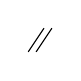
\begin{tikzpicture}[scale=0.2, baseline={([yshift=-0.5ex]current bounding box.center)}]  
			\draw[thin] (0,0) -- (1,1.5);  
			\draw[thin] (0.5,0) -- (1.5,1.5);  
		\end{tikzpicture}%  
	}%  
}  
\newcommand{\fourch}[4]
{\\[3pt]
	\begin{tabular}
		{*{4}{@{}p{4cm}}}
		A.~#1 & B.~#2 & C.~#3 & D.~#4
	\end{tabular}	
}
\newcommand{\fourchh}[4]
{\\[5pt]
	\begin{tabular}
		{*{4}{@{}p{20cm}}}
		A.~#1 \\[5pt] B.~#2 \\[5pt] C.~#3 \\[5pt] D.~#4
	\end{tabular}	
}
\newcommand{\fourchhh}[4]
{\\[3pt]
	\begin{tabular}
		{*{4}{@{}p{7.5cm}}}
		A.~#1 & B.~#2 \\[2pt] C.~#3 & D.~#4
	\end{tabular}	
}
\newcommand{\independent}{\perp\!\!\!\perp}
\everymath{\displaystyle}
\allowdisplaybreaks




\begin{document}
\tdplotsetmaincoords{70}{110} 
\pagestyle{fancy}
\lhead{Lecture 3}
\chead{illusion \& FzRainD}
\rhead{\today}
	
\setcounter{section}{2}


\section{相抵关系下的全系不变量\(-\)秩}

本节我们回到 \S 1 中留下的问题,我们对矩阵秩的定义还停留在简化行阶梯形矩阵,但我们已经发现这个定义有点太严格了,即使两个矩阵不能通过初等行变换互相得到,也可能有相同的秩. 沿着这条线索,我们同时采用两种初等变换对矩阵打洞化简,也就是我们本节所研究的相抵关系. 

\subsection{相抵关系及其全系不变量}

\subsubsection{相抵标准型}

假设我们现在已经得到了矩阵 \( A \in \F\nm \) 的简化行阶梯形矩阵,现在用列互换变换将主元调整至 \( 1 \sim r(A)=:r \) 列,也就得到如下的分块矩阵
\[ \begin{bmatrix}
	E_r & A_1 \\
	O & O
\end{bmatrix} \]

接下来,我们可以用第一列消去第一行 \( r \sim m \) 列的所有非零元,然后用第二列消去第二行 \( r \sim m \) 列的所有非零元,以此类推,将 \( A_1 \) 全部打洞为 \( O \). 或者也可以直接用如下的分块初等变换
\[ \begin{bmatrix}
	E_r & A_1 \\
	O & O
\end{bmatrix}\begin{bmatrix}
E_r & -A_1 \\
O & E_{m-r}
\end{bmatrix}=\begin{bmatrix}
E_r & O \\
O & O
\end{bmatrix}. \]

由于所用的分块初等矩阵是可逆的,那么必定可以分解为若干初等矩阵的乘积,也就相当于对列进行了若干次初等变换,本质上和第一种方法没什么区别. 可以发现,在这个过程中,矩阵的非零行数目没有任何改变,也就是先前我们定义的秩没有改变. 另一方面,我们得到了一种途径,仅通过初等变换将矩阵 \( A \) 变为对角矩阵 \( \diag\{E_r,O\} \),且主对角线上非零元素的个数恰好为矩阵的秩. 

问题自然而然地出现了. 

如果我们选择不同的初等变换方法将矩阵 \( A \) 化为主对角元素全为 \( 1,0  \) 的对角矩阵 (元素为 1 是很容易办到的,如果已经是对角矩阵,对非 1 的非零元素直接倍法变换即可),那么矩阵的秩会发生改变吗? 这个问题非常类似我们对简化行阶梯形矩阵的唯一性提出的问题. 

另一方面,注意到最后的这个矩阵它的非零子式的最大阶数恰好为 \( r \),这一点和简化行阶梯形矩阵没什么区别,简化行阶梯形矩阵的非零子式的最大阶数也为 \( r \). 于是猜测,原先的矩阵 \( A \) 的非零子式的最大阶数是否也是 \( r \) 呢?

接下来的讨论,就完美回答了这两个问题.

\begin{definition}[矩阵的相抵]
	称两个同型矩阵 \( A,B \in \F\nm \) 是相抵的,如果 \( A \) 可以经过有限次初等变换变为 \( B \). 用矩阵的语言,即存在 \( P \in \gfn, \; Q \in \gfm \) 使得 \( PAQ=B \),也记为 \( A \simeq B \).
\end{definition}

\begin{definition}[相抵标准形]
	由前述讨论可以看出,任意的矩阵 \( A \in \F\nm \) 必定可以相抵到如下形式的矩阵
	\[ \begin{bmatrix}
		E_r & O \\
		O & O
	\end{bmatrix}, \]
	
	称为 \( A \) 在相抵关系下的标准形.
\end{definition}

\begin{defprop}[秩的等价定义 I] \label{3.1.3}
	给定 \( A \in \F\nm \),若存在 \( P_1,P_2 \in \gfn, \; Q_1,Q_2 \in \gfm \) 使得
	\[ P_1AQ_1=\begin{bmatrix}
		E_r & O \\
		O & O
	\end{bmatrix}, \; P_2AQ_2=\begin{bmatrix}
	E_s & O \\
	O & O
	\end{bmatrix}, \]
	
	则必有 \( r=s \). 此时定义 \( r:=r(A) \) 为矩阵 \( A \) 的秩 (Rank).
\end{defprop}

\begin{proof}
	不妨 \( r<s \). 由于
	\[ P_1^{-1}\begin{bmatrix}
		E_r & O \\
		O & O
	\end{bmatrix}Q_1^{-1}=P_2^{-1}\begin{bmatrix}
	E_s & O \\
	O & O
	\end{bmatrix}Q_2^{-1}. \]
	
	记 \( M=P_2P_1^{-1}, \; N=Q_2^{-1}Q_1 \). 对 \( M,N \) 作如下分块
	\[ M=\begin{bNiceMatrix}[first-col,first-row]
		& r & m-r \\
		r & M_{11} & M_{12} \\
		n-r & M_{21} & M_{22}
	\end{bNiceMatrix}, \; N=\begin{bNiceMatrix}[first-col,first-row]
	& s & m-s \\
	s & N_{11} & N_{12} \\
	n-s & N_{21} & N_{22}
	\end{bNiceMatrix}. \]
	
	那么
	\[ \begin{bNiceMatrix}[first-col,first-row]
		& r & n-r \\
		r & M_{11} & M_{12} \\
		n-r & M_{21} & M_{22}
	\end{bNiceMatrix}\begin{bmatrix}
	E_r & O \\
	O & O
	\end{bmatrix}= \begin{bmatrix}
	E_s & O \\
	O & O
	\end{bmatrix}\begin{bNiceMatrix}[first-col,first-row]
	& s & m-s \\
	s & N_{11} & N_{12} \\
	m-s & N_{21} & N_{22}
	\end{bNiceMatrix}. \]
	
	计算可得
	\[ \begin{bNiceMatrix}[first-col,first-row]
		& r & n-r \\
		r & M_{11} & O \\
		n-r & M_{21} & O
	\end{bNiceMatrix}=\begin{bNiceMatrix}[first-col,first-row]
	& s & m-s \\
	s & N_{11} & N_{12} \\
	m-s & O & O
	\end{bNiceMatrix}. \]
	
	那么 \( N_{11}=(M_{11},O_{r \times (s-r)}) \, N_{12}=O \). 也就是
	\[ N=\begin{bNiceMatrix}[first-col,first-row]
		& s & m-s \\
		s & (M_{11},O_{r \times (s-r)}) & O \\
		m-s & N_{21} & N_{22}
	\end{bNiceMatrix}. \]
	
	注意 \( N \) 可逆,那么 \( N \) 的列向量组线性无关. 进一步,\( N \) 的第 \( (r+1) \sim m \) 列线性无关,但是 \( N \) 的第 \( (r+1) \sim m \) 列前 \( s \) 行的元素均为零,可视为 \( \F^{m-s} \) 中的列向量,但 \( m-r>m-s \),说明 \( N \) 的第 \( (r+1) \sim m \) 列必定线性相关,矛盾. 故 \( r \geq s \),对 \( r>s \) 同理推出矛盾,只能 \( r=s \).
	
	现在来证明秩定义的等价性. 如果我们用简化行阶梯矩阵的非零行数目来定义秩,计算
	\[ P_1A=\begin{bmatrix}
		E_r & O \\
		O & O
	\end{bmatrix}\begin{bmatrix}
	Q_{11} & Q_{12} \\
	Q_{21} & Q_{22}
	\end{bmatrix}=\begin{bmatrix}
	Q_{11} & Q_{12} \\
	O & O
	\end{bmatrix}. \]
	
	留意到 \( Q \) 的前 \( r \) 行必定线性无关. 那么对分块矩阵 \( (Q_{11},Q_{12})=(\alpha_1\T,\cdots,\alpha_r\T)\T \) 实行 Guass-Jordan 消元法不可能出现零行,若第 \( i \) 行被打为零行,意味着存在不全为零的数 \( c_1,\cdots,c_r \in \F \),使得
	\[ c_1\alpha_1+\cdots+c_r\alpha_r=\bm{0}. \]
	
	因为零行的出现只能由倍法变换和消法变换导致,这就相当于行向量的线性组合. 但这说明 \( Q \) 的前 \( r \) 行线性相关,矛盾. 故 \( P_1A \) 的简化行阶梯形矩阵的非零行数目也是 \( r \). 反之,若 \( A \) 的简化行阶梯形矩阵的非零行数目是 \( r \),那么必定可以再经过列初等变换化到 \( \diag\{E_r,O \} \).  也就说明了定义的等价性.
\end{proof}

\begin{proposition}[相抵关系为等价关系] \label{3.1.4}
	集合 \( \F\nm \) 上的相抵关系 \( \simeq \) 为等价关系,即其满足
	\begin{enumerate}[(1)]
		\item \textbf{反身性} \ \( A \simeq A \);
		\item \textbf{对称性} \ \( A \simeq B \) 蕴含 \( B \simeq A \);
		\item \textbf{传递性} \ \( A \simeq B \) 以及 \( B \simeq C \) 蕴含 \( A \simeq C \).
	\end{enumerate} 
\end{proposition}

\begin{proof}
	(1) \( E_nAE_m=A \); (2) \( PAQ=B \leadsto A=P^{-1}BQ^{-1} \); (3) \( PAQ=B, \; UBV=C \leadsto (UP)A(QV)=C \). 且可逆矩阵的乘积仍然可逆.
\end{proof}

我们回忆在基的定向曾经定义过的等价类的概念.

\begin{definition}[等价类]
	设 \( \sim \) 为集合 \( A \) 上的一个等价关系,那么称 \( A \) 的一个非空子集 \( C \) 为一个等价类,若
	\begin{enumerate}[(1)]
		\item \( C \) 中的元素相互等价,即对任意 \( x,y \in C \) 都有 \( x \sim y \);
		\item \( C \) 对 \( \sim \) 封闭,即对 \( x \in C, y \in A \),若 \( x \sim y \),那么 \( y \in C  \).
	\end{enumerate}
\end{definition}

\begin{proposition} \label{3.1.6}
	集合 \( \F\nm \) 上的相抵关系 \( \simeq \) 为等价关系,那么 \( \F\nm \) 可以分解为 \( \min\{n,m\}+1 \) 个等价类的无交并,每个等价类的代表元选取为其中矩阵的相抵标准形.
\end{proposition}

\begin{proof}
	先证明两个等价类要么相等,要么无交. 任取 \( C_1,C_2 \subseteq  \F\nm  \) 为两个等价类. 若 \( C_1 \cap C_2 \neq \emptyset \),取 \( Z \in C_1 \cap C_2 \). 那么任取 \( X \in C_1, \; Y \in C_2 \) 就有 \( X \simeq Z, \; Y \simeq Z \). 由对称性知 \( Z \simeq Y \),那么由传递性可知 \( X \simeq Y \). 由于 \( C_1, C_2 \) 对 \( \simeq \) 封闭,只好 \( X \in C_2, Y \in C_1 \). 这就说明了 \( C_1 \) 和 \( C_2 \) 相互包含,即 \( C_1=C_2 \).
	
	其次,对 \( A \in \F\nm \)定义 \( C_A:=\{X \in \F\nm \mid X \simeq A \} \). 首先由于反身性,\( A \in C_A \),说明 \( C_A \) 非空. 由于对称性和传递性可证 \( C_A \) 中的元素相互等价,以及 \( C_A \) 对 \( \simeq \) 封闭. 这说明 \( \F\nm \) 中每个元素都在某个等价类中,也就是 \( \F\nm \) 是等价类的并,而两个等价类要么相等,要么无交,说明  \( \F\nm \) 是等价类的无交并.
	
	由于每一个矩阵的相抵标准形是唯一的,且属于某个等价类中. \( \F\nm \) 中的相抵标准形一共只有  \( \min\{n,m\}+1 \) 种,说明无交的等价类也只有   \( \min\{n,m\}+1 \) 种.
\end{proof}

\begin{proposition} 
	设 \( A,B \in \F\mn \),那么 \( A \simeq B \) 当且仅当 \( r(A)=r(B) \). 即秩为相抵关系下的全系不变量. 相抵矩阵有相同的秩,反之亦然,有相同秩的矩阵必定相抵.
\end{proposition}

\begin{proof}
	\( r(A)=r(B) \) 当且仅当 \( A,B \) 有相同的相抵标准形,不妨设为 \( \Lambda \). 也就存在 \( P_1,P_2 \in \gfn, \; Q_1,Q_2 \in \gfm \) 使得 \( P_1AQ_1=P_2BQ_2=\Lambda \). 则 \( P_2^{-1}P_1AQ_1Q_2^{-1}=B \leadsto A \simeq B \). 或者也可以直接由 \( A \simeq \Lambda \simeq B \),结合命题 \ref{3.1.4} 的传递性得到.
\end{proof}

为了引出秩的子式定义,我们先证明一个引理.

\begin{lemma} \label{3.1.8}
	设 \( A \in \F\nm \),那么对 \( A \) 进行有限次初等变换不改变 \( A \) 非零子式的最大阶数.
\end{lemma}

\begin{proof}
	 \( A \neq O \) 是平凡的. 设 \( A \) 的非零子式的最大阶数为 \( r (1 \leq r \leq n) \). 下面只讨论行初等变换的情况,由于转置不改变行列式的值,所以列初等变换的情况可以化归到行初等变换来考虑. 
	 
	 由于初等变换是可逆的,那么如果 \( A \) 能初等变换变为 \( B \),那么 \( B \) 也能经过初等变换变为 \( A \). 只要证明 \( B \) 的非零子式的最大阶数不低于 \( A \) 的非零子式的最大阶数. 因为反之也必定成立,就得出结论. 注意到互换变换可以分解为倍法变换和消法变换的复合,即
	 \[ E(i,j)=E(j(-1))E(i,j(1))E(j,i(-1))E(i,j(1)). \]
	 
	 那么我们只讨论倍法变换和消法变换的情形. 对倍法变换,如果将第 \( i \) 行乘以非零常数 \( c \neq 0 \),如果 \( A \) 的 \( r \) 阶非零子式包含第 \( i \) 行,那么只会变为原来的 \( c \) 倍,若不包含第 \( i \) 行,则其值不变. 即 \( A \) 经过一次行倍法变换得到 \( B \) 后,\( B \) 也必定存在 \( r \) 阶非零子式.
	 
	 对消法变换,将第 \( i \) 行乘以常数 \( c \) 加到第 \( j \) 行. 如果 \( A \) 的 \( r \) 阶非零子式同时包含第 \( i,j \) 行或不包含第 \( j \) 行,其值不变. 若只包含第 \( j \) 行. 用 \( M_r \neq 0  \) 表示这个非零子式,\( L_r \) 表示 \( M_r \) 中包含的 \( A \) 第 \( j \) 行用第 \( i \) 行元素替代,\( N_r \) 表示 \( M_r \) 中包含的 \( A \) 第 \( j \) 行是实行消法变换后的. 若 \( L_r=0 \),那么由行列式性质知 \( N_r=cL_r+M_r=M_r \neq 0 \).若 \( L_r \neq 0 \),那么 \( A \) 中原本就包含一个值为 \( \pm L_r \) 的子式,它没有参与消法变换,自然也是 \( B \) 中的一个 \( r \) 阶非零子式.
\end{proof}

\begin{defprop}[秩的等价定义 II] \label{3.1.9}
	设 \( A \in \F\nm \),若 \( A \) 存在一个 \( r \) 阶子式非零,且若其存在 \( (r+1) \) 阶子式,那么 \( A \) 的所有  \( (r+1) \) 阶子式全为零,则称矩阵 \( A \) 的秩 (Rank) 为 \( r(A):=r \).
\end{defprop}

\begin{proof}
	若秩采用定义\(-\)命题 \ref{3.1.3} 定义,设 \( r(A)=r \),则 \( A \) 的相抵标准形为 \( \diag\{E_r,O\} \),而由引理 \ref{3.1.8} 知道初等变换不改变非零子式的最大阶数,而相抵标准形非零子式的最大阶数为 \( r \). 
	
	反之,若秩采用定义\(-\)命题 \ref{3.1.9},设 \( r(A)=r \),以及 \( A \) 的相抵标准形为 \( \diag\{E_s,O\} \),再由引理 \ref{3.1.8} 知道它的非零子式的最高阶数为 \( s=r \).
\end{proof}

\begin{corollary} \label{3.1.10}
	命题 \ref{3.1.6} 和引理 \ref{3.1.8} 共同说明了初等变换不改变矩阵的秩. 用矩阵的语言即,对 \( A \in \F\mn \),以及 \( P \in \gfm, \; Q \in \gfn \) 都有 \( r(A)=r(PA)=r(AQ)=r(PAQ) \).
\end{corollary}

\begin{proof}
	命题 \ref{3.1.6} 说明初等变换前后的矩阵在同一个等价类中,有相同的相抵标准形,那么由定义\(-\)命题 \ref{3.1.3} 说明秩相同. 引理 \ref{3.1.8} 说明初等变换不改变非零子式的最大阶数, 由定义\(-\)命题 \ref{3.1.9} 说明秩相同. 这两个定义是自恰的.
\end{proof}

在定义\(-\)命题 \ref{3.1.9} 中的条件还可以进行削弱. 有如下的命题:

\begin{proposition} \label{3.1.11}
	设 \( A \in \F\nm \),若 \( A \) 存在一个 \( r \) 阶子式非零,且若其存在 \( (r+1) \) 阶子式,且包含这个非零 \( r \) 阶子式的 \( r+1 \) 阶子式全为零,那么 \( r(A)=r \).
\end{proposition}

\begin{proof}
	避免角标的繁琐讨论,不妨设这个非零 \( r \) 阶子式即 \( A \) 的 \( r \) 阶顺序主子式
	\[ A\begin{bmatrix}
		1 & 2 & \cdots & r \\
		1 & 2 & \cdots & r
	\end{bmatrix}, \]
	
	设 \( A=(\alpha_1,\cdots,\alpha_m) \). 对 \( \alpha_1,\cdots,\alpha_r \) 取它们的前 \( r \) 部分分量构成的缩短向量 \( \widetilde{\alpha}_1, \cdots, \widetilde{\alpha}_r \). 由于 \( A \) 的 \( r \) 阶顺序主子式非零,即对应的矩阵可逆,那么 \( \widetilde{\alpha}_1, \cdots, \widetilde{\alpha}_r  \) 线性无关. 考察 \( c_1\alpha_1+\cdots+c_r\alpha_r=\bm{0} \),取这个等式的前 \( r \) 分量即 \( c_1\widetilde{\alpha}_1,+\cdots+c_r\widetilde{\alpha}_r=\bm{0} \). 那么只能 \( c_1=\cdots=c_r=0 \). 我们断言 \( \alpha_{r+1},\cdots,\alpha_m \) 可以被 \( \alpha_1,\cdots,\alpha_r \) 线性表出,否则,存在 \( \alpha_t \ (r+1 \leq t \leq m) \) 不能被  \( \alpha_1,\cdots,\alpha_r \) 线性表出,那么 \( \alpha_1,\cdots,\alpha_r,\alpha_t \) 线性无关. 取包含 \( r \) 阶顺序主子式以及第 \( t \) 列构成的加边 \( r+1 \) 阶子式,显然这个子式对应的矩阵可逆,那么子式的值非零,与题设矛盾.
	
	现在对 \( A \) 的列执行 Guass-Jordan 消元法,那么 \( (r+1) \sim m \) 列会被 \( 1 \sim r \) 列的线性组合打成 \( \bm{0} \). 由于 \( A \) 左上方的 \( r \) 阶矩阵块可逆,因为 \( r \) 阶顺序主子式非零,那么列初等变换会直接将这个矩阵变为 \( E_r \),也就是存在 \( Q \in \gfm \),使得
	\[ AQ=\begin{bmatrix}
		E_r & O \\
		A_1 & O
	\end{bmatrix} \leadsto \begin{bmatrix}
	E_r & O \\
	-A_1 & E_{n-r}
	\end{bmatrix}AQ=\begin{bmatrix}
	E_r & O \\
	O & O
	\end{bmatrix}. \]
	
	由定义\(-\)命题 \ref{3.1.3} 可知 \( r(A)=r \).
\end{proof}

\begin{remark}
	从命题 \ref{3.1.6} 或者定义\(-\)命题 \ref{3.1.9} 中我们轻易读取出秩的粗略范围 \( 0 \leq r(A) \leq \min\{\text{column}(A), \text{row}(A) \} \). 这是不言而喻的. 另一方面,由于转置不改变行列式的值,那么 \( r(A)=r(A\T) \).
\end{remark}

\subsubsection{秩不等式}

到此为止,我们对秩有三种等价定义: 非零子式的最大阶数,(简化)行阶梯形矩阵的非零行数目,相抵标准形中对角线上 1 的个数. 除了用这些定义,解决秩有关的问题还会频繁使用到推论 \ref{3.1.10},也就是对原矩阵进行合适的初等变换,使得我们能够容易读取出秩的信息,例如我们从(简化)行阶梯形矩阵的非零行数目读取秩就是利用了这一点.

除了这些基本的原理外,我们还需要一些额外的工具,在此我们总结为一些常用秩不等式,需要熟练掌握. 除了在本节所述的方法外,我们未来在 \S 5 中还会用向量组的极大线性无关组理论以及 \S 6 齐次线性方程组的基础解系理论给出一些别的证明.

必须强调的是,初等变换方法和考虑相抵关系下的代表元这两个思想可以说贯穿高等代数的学习生涯,需要足够的重视,你马上会看到我们花费大量笔墨描述等价关系,等价类的用处.

\begin{proposition} \label{3.1.13}
	设 \( A \in \F\nm, \; B \in \F^{m \times t} \),那么 \( r(AB) \leq \min\{r(A),r(B)\} \).
\end{proposition}

\begin{proof}
	(\textbf{法一}) \ 由于初等变换不改变秩,也就不改变原命题的表述. 不妨一开始就设 \( A \mapsto PAQ= \diag\{E_r,O\} \), \( B \mapsto Q^{-1}B \). 这样进行 \( B \) 的变换不会改变 \( B \) 选取的任意性和 \( B \) 的秩. 于是再设
	
	\[
	B =\begin{bmatrix}
		B_{11} & B_{12} \\
		B_{21} & B_{22}
	\end{bmatrix} \leadsto AB =\begin{bmatrix}
		E_r & O \\
		O   & O
	\end{bmatrix}\begin{bmatrix}
		B_{11} & B_{12} \\
		B_{21} & B_{22}
	\end{bmatrix}=\begin{bmatrix}
		B_{11} & B_{12} \\
		O      & O
	\end{bmatrix}.
	\]
	
	这说明 \( AB \) 至多有 \( r \) 阶非零子式,于是 \( r(AB) \leq r=r(A) \). 如果我们一开始设 \( A \mapsto AP^{-1}, \; B \mapsto PBQ=\diag\{E_s,O\} \),那么就能得到 \( r(AB) \leq s=r(B) \).
	
	\vspace{1ex}
	
	(\textbf{法二})\ 设 \( r(A)=r \),利用 Cauchy\(-\)Binet 公式,得到
	\[ AB\begin{bmatrix}
		i_1 & i_2 & \cdots & i_s \\
		j_1 & j_2 & \cdots & j_s
	\end{bmatrix}= \sum_{1 \leq l_1 < \cdots < l_s \leq n}^{} A\begin{bmatrix}
	i_1 & i_2 & \cdots & i_s \\
	l_1 & l_2 & \cdots & l_s
	\end{bmatrix} A\begin{bmatrix}
	l_1 & l_2 & \cdots & l_s\\
	j_1 & j_2 & \cdots & j_s
	\end{bmatrix}. \]
	
	当 \( s>r \) 时,关于 \( A \) 的子式那一项都是 0,最后求和的结果也必然是 0. 于是 \( r(AB) \leq r=r(A) \). 同理 \( r(AB) \leq r(B) \). 
	
	\vspace{1ex}
	
	(\textbf{法三})\ 可以看成法一的细化. 设 \( r(A)=r, r(B)=s \). 那么存在 \( P \in \gfn, \; Q, U \in \gfm, \; V \in \text{GL}_t(\F) \) 使得
	\[
	A = P
	\begin{bmatrix}
		E_r & O \\
		O   & O
	\end{bmatrix}
	Q, 
	\quad 
	B = U
	\begin{bmatrix}
		E_s & O \\
		O   & O
	\end{bmatrix}
	V.
	\]
	
	那么
	\[
	r(AB) = r \left(
	\begin{bmatrix}
		E_r & O \\
		O   & O
	\end{bmatrix}
	QU
	\begin{bmatrix}
		E_s & O \\
		O   & O
	\end{bmatrix}
	\right).
	\]
	
	接下来对 \( QU \) 分块,有
	\[
	QU =
	\begin{bmatrix}
		C_{11} & C_{12} \\
		C_{21} & C_{22}
	\end{bmatrix}
	\leadsto
	\begin{bmatrix}
		E_r & O \\
		O   & O
	\end{bmatrix}
	QU
	\begin{bmatrix}
		E_s & O \\
		O   & O
	\end{bmatrix}
	=
	\begin{bmatrix}
		C_{11} & O \\
		O & O
	\end{bmatrix}.
	\]
	
	但 \( C_{11} \in \F^{r \times s} \),说明 \( r(A)=r(C_{11}) \leq \min\{r,s\} \).
	
\end{proof}

\begin{proposition} \label{3.1.14}
	设 \( A \in \F\mn, \; B \in \F^{t \times p} \),任取 \( C \in \F^{m \times p}\),那么
	\[ r \begin{bmatrix}
		A & O \\ O & B
	\end{bmatrix}=r(A)+r(B), \; r \begin{bmatrix}
	A & C \\ O & B
	\end{bmatrix} \geq r(A)+r(B). \]
\end{proposition}

\begin{proof}
	(\textbf{法一})\ 设 \( r(A)=r, \; r(B)=s \). 那么存在 \( P \in \gfm, \; Q \in \gfn, \; U \in \text{GL}_t(\F), \; V \in \text{GL}_p(\F) \),使得
	\[ PAQ=\begin{bmatrix}
		E_r & O \\ O & O
	\end{bmatrix}, \; UBV=\begin{bmatrix}
	E_s & O \\ O & O
	\end{bmatrix}. \]
	
	用分块矩阵来写就是
	\[ \begin{bmatrix}
		P & O \\ O & U
	\end{bmatrix}\begin{bmatrix}
	A & O \\ O & B
	\end{bmatrix}\begin{bmatrix}
	Q & O \\ O & V
	\end{bmatrix}=\begin{bmatrix}
	PAQ & O \\ O & UBV
	\end{bmatrix}=\begin{bmatrix}
	E_r & O & O & O \\ O & O & O & O \\ O & O & E_s & O \\ O & O & O & O 
\end{bmatrix}. \]

进行适当的互换变换
\[ \begin{bmatrix}
	E_r & O & O & O \\ O & O & O & O \\ O & O & E_s & O \\ O & O & O & O 
\end{bmatrix} \leadsto \begin{bmatrix}
E_r & O & O & O \\ O & E_s & O & O \\ O & O & O & O \\ O & O & O & O 
\end{bmatrix}. \]

于是第一个结论得证. 对第二个结论,再考虑 
\[ PCV=\begin{bmatrix}
	C_{11} & C_{12} \\
	C_{21} & C_{22}
\end{bmatrix} \leadsto \begin{bmatrix}
P & O \\ O & U
\end{bmatrix}\begin{bmatrix}
A & C \\ O & B
\end{bmatrix}\begin{bmatrix}
Q & O \\ O & V
\end{bmatrix}=\begin{bmatrix}
PAQ & PCV \\ O & UBV
\end{bmatrix}=\begin{bmatrix}
E_r & O & C_{11} & C_{12} \\ O & O & C_{21} & C_{22} \\ O & O & E_s & O \\ O & O & O & O 
\end{bmatrix}. \]

明显 \( E_r \) 能消去 \( C_{12} \); \( E_s \) 能消去 \( C_{11}, \; C_{21} \),稍微写一下分块矩阵的初等变换即可. 再进行适当的互换变换,就有
\[ \begin{bmatrix}
	E_r & O & C_{11} & C_{12} \\ O & O & C_{21} & C_{22} \\ O & O & E_s & O \\ O & O & O & O 
\end{bmatrix} \leadsto \begin{bmatrix}
E_r & O & O & O \\ O & E_s & O & O \\ O & O & C_{12} & O \\ O & O & O & O 
\end{bmatrix}. \]

那么至少有一个 \( r+s \) 阶非零子式,算上 \( C_{12} \) 可能能提供更高阶的非零子式,可惜我们不知道它的任何信息.

(\textbf{法二})\ 任取 \( \diag\{A,B\} \) 的一个非零 \( m \) 阶子式,它必定形如 \( \det \diag\{A_1,B_1\} \),其中 \( A_1,B_1 \) 分别为 \( A,B \) 的一个子矩阵,允许为零阶. 如果希望 \( \det \diag\{A_1,B_1\}=\det A_1 \det B_1 \neq 0 \),那么 \( \det A_1, \; \det B_1 \) 也分别为 \( A, B \) 的非零子式. 而它们具有非零子式的最高阶数分别为 \( r(A), \; r(B) \). 从而 \( \diag\{A,B\} \) 非零子式的最高阶数即 \( r(A)+r(B) \),那么由定义\(-\)命题 \ref{3.1.9} 知第一个结论即证. 对第二个结论,取 \( A \) 的 \( r(A) \) 阶非零子式 \( A_1 \) 以及 \( B \) 的 \( r(B) \) 阶非零子式 \( B_1 \). 这两者对应
\[ \begin{bmatrix}
	A & C \\ O & B
\end{bmatrix} \]

一个非零子式
\[ \det \begin{bmatrix}
	A_1 & C_1 \\ O & B_1
\end{bmatrix} = \det A_1 \det B_1 \neq 0, \]

于是第二个结论即证.

\end{proof}

命题 \ref{3.1.14} 的取等条件和某一类方程是否有解有关,也就是下面的 Roth 定理. 

\begin{theorem}[Roth] \label{3.1.15}
	在命题 \ref{3.1.14} 的条件下,设 \( X \in \F^{n \times p}, \; Y \in \F^{m \times t} \),那么矩阵方程 \( AX-YB=C \) 有解的充分必要条件为
	\[ r\begin{bmatrix}
		A & O \\ O & B
	\end{bmatrix}= r\begin{bmatrix}
		A & C \\ O & B
	\end{bmatrix}= r(A)+r(B). \]
\end{theorem}

\begin{proof}
	先证明充分性. 首先复述命题 \ref{3.1.14} 法一的所有过程,我们将所用的分块矩阵初等变换写出,即
	\[ \begin{bmatrix}
		E_r & O & -C_{11} & O \\
		O & E_{m-r} & -C_{21} & O \\
		O & O & E_s & O \\
		O & O & O & E_{t-s}
	\end{bmatrix} \begin{bmatrix}
		E_r & O & C_{11} & C_{12} \\
		O & O & C_{21} & C_{22} \\
		O & O & E_s & O \\
		O & O & O & O
	\end{bmatrix}\begin{bmatrix}
		E_r & O & O & -C_{12} \\
		O & E_{n-r} & O & O \\
		O & O & E_s & O \\
		O & O & O & E_{p-s}
	\end{bmatrix}=\begin{bmatrix}
		E_t & O & O & O \\
		O & O & O & C_{22} \\
		O & O & E_s & O \\
		O & O & O & O
	\end{bmatrix}.  \]
	
	那么这时候希望 \( C_{22}=O \),否则必然存在一个 \( r+s+1 \) 阶非零子式.令
	\[ R_1= \begin{bmatrix}
		C_{11} & O \\ C_{21} & O
	\end{bmatrix}, \; R_2=\begin{bmatrix}
		O & C_{12} \\ O & O 
	\end{bmatrix}. \]
	
	那么
	\[ \begin{bmatrix}
		E_n & -R_1 \\ O & E_t
	\end{bmatrix}\begin{bmatrix}
		PAQ &  PCV \\ O & UBV
	\end{bmatrix}\begin{bmatrix}
		E_n & -R_2 \\ O & E_p
	\end{bmatrix}=\begin{bmatrix}
		E_t & O & O & O \\
		O & O & O & O \\
		O & O & E_s & O \\
		O & O & O & O
	\end{bmatrix}. \]
	
	计算左端的展开,
	\[ \begin{bmatrix}
		E_n & -R_1 \\ O & E_t
	\end{bmatrix}\begin{bmatrix}
		PAQ &  PCV \\ O & UBV
	\end{bmatrix}\begin{bmatrix}
		E_n & -R_2 \\ O & E_p
	\end{bmatrix}=\begin{bmatrix}
	PAQ &  -PAQR_2+PCV-R_1UBV \\ O & UBV
	\end{bmatrix}. \]
	
	就得到 \( PA(QR_2)+(R_1U)BV=PCV \leadsto A(QR_2V^{-1})-(-P^{-1}R_1U)B=C \). 再证明必要性,这是非常容易的,设 \( X_0 \in \F^{n \times p}, \; Y_0 \in \F^{m \times t} \) 满足 \( AX_0-Y_0B=C \). 那么直接分块矩阵的初等变换就得到
	\[ \begin{bmatrix}
		E_m & -Y_0 \\ O & E_t
	\end{bmatrix}\begin{bmatrix}
		A & O \\ O & B
	\end{bmatrix}\begin{bmatrix}
	E_n & X_0 \\ O & E_p
	\end{bmatrix}=\begin{bmatrix}
		A & C \\ O & B
	\end{bmatrix}. \]
	
	而初等变换不改变矩阵的秩,得证.
	
\end{proof}

\begin{proposition}[Sylvester] \label{3.1.16}
	设 \( A \in \F\nm, \; B \in \F^{m \times t} \),那么 \( r(AB) \geq r(A)+r(B)-m \). 特别地,若 \( AB=O \),那么 \( r(A)+r(B) \leq m \).
\end{proposition}

\begin{proof}
	只需证 \( r(AB)+r(E_m) \geq r(A)+r(B) \). 作如下的分块矩阵初等变换
	\[ \begin{bmatrix}
		AB & O \\ O & E_m
	\end{bmatrix} \leadsto \begin{bmatrix}
	AB & -A \\ O & E_m
	\end{bmatrix} \leadsto \begin{bmatrix}
	O & -A \\ B & E_m
	\end{bmatrix} \leadsto \begin{bmatrix}
	 B & E_m \\ O & A
	\end{bmatrix}. \]
	
	由命题 \ref{3.1.14} 即得. 
\end{proof}

\begin{corollary}
	命题 \ref{3.1.16},Sylvester 不等式取等当且仅当 \( BX-YA=E_m \) 有解.
\end{corollary}

\begin{proof}
	从命题 \ref{3.1.16} 的证明可以读出就是命题 \ref{3.1.14} 当 \( C=E_m \) 的取等条件. 应用 Roth 定理即可,即定理 \ref{3.1.15}. 
\end{proof}

下面的 Frobenius 不等式是对 Sylvester 不等式的推广,Sylvester 不等式就是 Frobenius 不等式在 \( B=E_m \) 的情况.

\begin{proposition}[Frobenius]
	设 \( A \in \F\nm, \; B \in \F^{m \times t}, \; C \in \F^{t \times p} \),那么 \( r(ABC) \geq r(AB)+r(BC)-n(B) \). 
\end{proposition}

\begin{proof}
	完全类似命题 \ref{3.1.16} 的证明. 作如下的分块矩阵初等变换
	\[ \begin{bmatrix}
		ABC & O \\ O & B
	\end{bmatrix} \leadsto \begin{bmatrix}
		ABC & -AB \\ O & B
	\end{bmatrix} \leadsto \begin{bmatrix}
		O & -AB \\ BC & B
	\end{bmatrix} \leadsto \begin{bmatrix}
		BC & B \\ O & AB
	\end{bmatrix}. \]
	
	当然也有类似的取等条件,此处略过.
\end{proof}

\begin{proposition} \label{3.1.19}
	设 \( A \in \F\nm, \; B \in \F^{n \times t} \),那么 \( r(A,B) \leq r(A)+r(B) \). 由于转置不改变秩,那么
	\[ r \begin{bmatrix}
		A \\ B
	\end{bmatrix} \leq r(A)+r(B). \]
\end{proposition}

\begin{proof}
	(\textbf{法一})\ 注意到
	\[ \begin{bmatrix}
		E_n & E_n
	\end{bmatrix}\begin{bmatrix}
		A & O \\ O & B
	\end{bmatrix}=(A,B), \]
	
	再利用命题 \ref{3.1.13} 即可.
	
	\vspace{1ex}
	
	(\textbf{法二})\ 设 \( r(A)=r \),那么存在 \( P \in \gfn, \; Q \in \gfm \) 使得 \( PAQ=\diag\{E_r,O\} \). 对 \( PB \) 按 \( PAQ \) 的形式分块,
	\[ PB=\begin{bmatrix}
		B_{11} & B_{12} \\
		B_{21} & B_{22}
	\end{bmatrix},\]
	
	也就说明存在如下的初等变换,
	\[ (A,B)=\begin{pmatrix}
		E_r & O & B_{11} & B_{12} \\
		O & O & B_{21} & B_{22}
	\end{pmatrix} \leadsto \begin{pmatrix}
	E_r & O & O & O \\
	O & O & B_{21} & B_{22}
	\end{pmatrix}. \]
	
	于是由命题 \ref{3.1.14} 知道 \( r(A,B)=r(E_r,O)+r(B_{21},B_{22}) \leq r+r(B) \).
\end{proof}

\begin{proposition} \label{3.1.20}
	设 \( A, B \in \F\nm \),那么 \( |r(A)-r(B)| \leq r(A\pm B) \leq r(A)+r(B) \). 
\end{proposition}

\begin{proof}
	(\textbf{法一})\ 先证明 \( r(A\pm B) \leq r(A)+r(B)  \). 设 \( r(A)=r, \; r(B)=s \). 那么存在 \( P_1,P_2 \in \gfn, \; Q_1,Q_2 \in \gfm \) 使得 \( A=P_1\diag\{E_r,O\}Q, \; B=P_2\diag\{E_s,O\}Q_2 \). 于是
	\[ A \pm B= (P_1,P_2)\diag\{E_r,O,\pm E_s,O\}(Q_1,Q_2)\T. \]
	
	利用命题 \ref{3.1.13} 得到 \( r(A \pm B) \leq r+s \). 另一方面,不妨设 \( r>s \),那么 \( r(A-B)+r(B) \geq r(A-B+B)=r(A) \),也就是 \( r(A-B) \geq r(A)-r(B)=|r(A)-r(B)| \). 另一方面,注意 \( r(B)=r(-B) \),那么 \( r(A+B) \geq r(A)-r(-B) \),代入即可.
	
	(\textbf{法二})\ 给出 \( r(A\pm B) \leq r(A)+r(B)  \) 的另一种证明. 注意到 \( A \pm B \) 所有的子式也都是分块矩阵
	\[ \begin{bmatrix}
		A & A \pm B \\ O & B
	\end{bmatrix} \]
	
	的子式,又该分块矩阵可以初等变换变为
	\[ \begin{bmatrix}
		A & A \pm B \\ O & B
	\end{bmatrix} \leadsto \begin{bmatrix}
	A & O \\ O & B
	\end{bmatrix}, \]
	
	那么 
	\[ r(A\pm B) \leq r\left( \begin{bmatrix}
		A & A \pm B \\ O & B
	\end{bmatrix} \right)=r\left( \begin{bmatrix}
	A & O \\ O & B
	\end{bmatrix} \right)=r(A)+r(B). \]	 
	
	(\textbf{法三})\ 熟知
	\[ (A,B)\begin{pmatrix}
		E_n \\ E_n
	\end{pmatrix}=A+B. \]
	
	那么由命题 \ref{3.1.13} 和命题 \ref{3.1.19} 得到 \( r(A+B) \leq r(A,B) \leq r(A)+r(B) \).
\end{proof}


\subsubsection{秩问题浅谈}

下面的例子基本离不开初等变换法. 这是一种需要你务必掌握的方法,再怎么强调都不为过.


\begin{example}
	设 \( A, B \in \F\n \),求证:\( r(AB) = r(BA) \) 的充要条件是  
	\[ r\left( \begin{bmatrix} E & A \\ B & O \end{bmatrix} \right) = r\left( \begin{bmatrix} E & B \\ A & O \end{bmatrix} \right). \]
\end{example}

\begin{proof}
	
\end{proof}



\begin{example}
	设 \(  A \in \F\n \). 证明:
	\begin{enumerate}[(1)]
		\item \( A^2=A \) 的充要条件为 \( r(A)+r(A-E)=n \);
		\item \( A^2=E \) 的充要条件为 \( r(A+E)+r(A-E)=n \);
		\item \( A^3=E \) 的充要条件为 \( r(A-E)+r(A^2+A+E)=n \);
		\item \( \cdots \)
	\end{enumerate}
	
	这一系列命题都来自互素多项式导出的空间直和分解,留给高等代数 II 探究其本质.
\end{example}

\begin{proof}
	
\end{proof}

\begin{example}
	设 \( A \in \gfn, \; B \in \F\mn, \; C \in \F\nm \). 求证  
	\( r(BA^{-1}C + E_m) < m \) 的充要条件是 \( r(A + CB) < n \).
\end{example}

\begin{proof}
	
\end{proof}


\begin{example}
	设 \(  A, B \in \F\n \) 满足 \( A + B = E \). 求证 \( r(A) + r(B) = n \) 的充要条件是  
	\( A^2 = A, B^2 = B \) 且 \( AB = BA = O \).
\end{example}

\begin{proof}
	
\end{proof}

主对角元严格行占优方阵必定可逆是一个经典的结论,它的想法就来自 Guass-Jordan 消元法. 当然,使用线性方程组理论可以给出一个漂亮的证明.

\begin{lemma}
	设 \( A = (a_{ij}) \in \F\n \) 主对角元严格行占优,即对于任意的 \( 1 \leq i \leq n \),均有
	\[
	|a_{ii}| > \sum_{j=1, j \neq i}^{n} |a_{ij}|.
	\]
	
	证明: \( r(A)=n \),即 \( A \) 可逆.
\end{lemma}

\begin{proof}
	
\end{proof}


\begin{example}
	设 \( A = (a_{ij}) \in \F\n \) 满足以下条件
	\begin{enumerate}[(i)]
		\item \( a_{ii} > 0 \),\( i = 1, 2, \cdots, n \);
		\item \( a_{ij} < 0 \),\( i \neq j \);
		\item \( \sum_{i=1}^{n} a_{ij} = 0 \),\( j = 1, 2, \cdots, n \).
	\end{enumerate}
	
	试求 \( r(A) \).
\end{example}

\begin{proof}
	
\end{proof}


下面的问题大多基于前面有关秩不等式的研究,如何熟练运用已知的不等式,需要多练习.

\begin{example}
	设 \( A \in \F\mn \),求证方程 \( AX = E_m \) 有解的充要条件是 \( r(A) = m \).
\end{example}

\begin{proof}
	
\end{proof}


\begin{example} \label{3.1.28}
	设 \(  A \in \F\mn, \; B \in \F^{n \times k} \). 
	\begin{enumerate}[(1)]
		\item 若 \( r(AB)=r(A) \),那么对任意 \( C \in \F^{t \times m} \) 都有 \( r(CAB)=r(CA) \);
		\item 若 \( r(AB)=r(B) \),那么对任意 \( C \in \F^{k \times l} \),都有 \( r(ABC)=r(BC) \).
	\end{enumerate}
\end{example}

\begin{proof}
	
\end{proof}

下面的例子是对例 \ref{3.1.28} 的推广.

\begin{example}
	设 \(  P_i,Q_i \in \F\n \ (1 \leq i \leq s) \) 满足任意的 \( 1 \leq i,j \leq s \) 都有 \( P_iQ_j=Q_jP_i \). 
	\begin{enumerate}[(1)]
		\item 若对任意 \( 1 \leq i \leq s \),都有 \( r(P_i)=r(P_iQ_i) \),那么
		\[ r(P_1\cdots P_s Q_1\cdots Q_s)=r(P_1\cdots P_s); \]
		\item 若对任意 \( 1 \leq i \leq s \),都有 \( r(Q_i)=r(P_iQ_i) \),那么
		\[ r(P_1\cdots P_s Q_1\cdots Q_s)=r(Q_1\cdots Q_s). \]
	\end{enumerate}
\end{example}

\begin{proof}
	
\end{proof}

\subsection{相抵标准型的应用}


\subsubsection{利用代表元处理问题的方法}


\subsubsection{秩一矩阵和降阶公式}

\begin{theorem}[秩和行列式的降阶公式 I]
	设 \( A \in \F\n, \; D \in \F^{m \times m} \) 以及 \( B \in \F\nm, \; C \in \F\mn \),考察分块矩阵
	\[ M:=\begin{bmatrix}
		A & B \\ C & D
	\end{bmatrix}. \]
	
	那么
	\begin{enumerate}[(1)]
		\item 若 \( A \in \gfn \),那么
		\[ \det M=\det A\det (D-CA^{-1}B), \; r(M)=r(A)+r(D-CA^{-1}B); \]
		\item 若 \( D \in \gfn \),那么
		\[ \det M=\det D\det (A-BD^{-1}C), \; r(M)=r(D)+r(A-BD^{-1}C). \]
	\end{enumerate}
\end{theorem}

\begin{proof}
	
\end{proof}

\begin{example}
	设 \( A,B,C,D \in \F\n \),记其行列式分别为 \( a,b,c,d \). 设
	\[ r\begin{bmatrix}
		A & B \\ C & D
	\end{bmatrix}=n, \]
	
	证明: \( ad=bc \). 且若 \( A \) 可逆,则 \( D=CA^{-1}B \).
\end{example}

\begin{proof}
	
\end{proof}

\begin{theorem}[特征值的降阶公式]
	设 \( A \in \F\nm, \; B \in \F\mn \),\( k \) 为给定常数. 那么
	\[ \lambda^m \det(\lambda E_n - AB)= \lambda^{n} \det(\lambda E_m - BA). \]
\end{theorem}

\begin{proof}
	
\end{proof}

\begin{corollary}[行列式的降阶公式 II]
	设 \( A \in \F\nm, \; B \in \F\mn \). 那么
	\[ \det(E_n - AB)= \det(E_m - BA). \]
\end{corollary}

\begin{proof}
	
\end{proof}

\subsubsection{一些计算实例 III}


\subsubsection{行满秩和列满秩矩阵}


\subsubsection{矩阵的满秩分解}



\subsection{特殊的相抵关系: 合同与相似}

\subsubsection{合同与相似初等变换}


\subsubsection{实反对称阵}


\subsubsection{幂零矩阵}


\subsubsection{幂等矩阵}


\subsubsection{对合矩阵}


\end{document}
